\documentclass[10pt]{article}
\usepackage{icmlko}

\icmlmeta{IP 파운데이션 월드모델}{60}{인코더를 만들어 겨뤘고 졌다}{공유 인코더에 도메인별 헤드 --- 프론티어 쪽 구성을 같은 규약으로 세웠더니 닫힌 해가 두 배 앞선다}

\begin{document}

\twocolumn[
\icmlheader

\begin{abstract}
현행 파이프라인은 도메인마다 주성분 둘을 뽑고 쌍마다 프로크루스테스로 회전을
맞춘다 --- 정렬이 \emph{닫힌 해}로 계산되고 학습되지 않는다. 다중 도메인 모델의
표준 구성은 다르다. 모든 도메인이 \textbf{공유 인코더}를 통과해 같은 잠재
공간에 놓이고 도메인마다 얇은 헤드만 따로 둔다. 그 구조를 같은 규약으로 세워
겨뤘다 --- 입력은 다섯 축 값과 다섯 마스크, 잠재 차원은 둘(현행과 용량을 맞춤),
평가는 출처 헤드를 대상 잠재에 적용해 순위 상관. \textbf{졌다.} 현행 선형이
$+$0.3506인데 공유 인코더는 $+$0.1702$\pm$0.0178, 출처 하나로만 학습하면
$+$0.1630$\pm$0.0091이다. 차이가 씨앗 표준편차의 10--20배라 \textbf{판정이
가능한 패배}다 --- 노트 14에서 신경망 씨앗 분산이 효과의 4--5배라 아무것도
말할 수 없었던 것과 달라졌고, 표본이 커진 덕이다. 원인을 두 번 짚었다.
첫째 가설은 ``프로크루스테스는 도메인별 회전을 자유롭게 두는데 공유 인코더는
하나로 강제한다''였고, 도메인별 사영을 앞에 붙여 검정하니 $+$0.1665로
\textbf{변화가 없어 기각}됐다. 둘째로 신경망 잠재에 프로크루스테스를 붙이니
$+$0.2004로 \textbf{부분 회복}한다. 즉 \textbf{표현과 정렬 둘 다에서 진다} ---
정렬을 되돌려 받아도 $+$0.03만 회복하고 나머지 $+$0.15는 표현 자체의 차이다.
\end{abstract}
]

\section{같은 규약으로 세웠다}

다중 과제 학습의 표준 구성을 그대로 옮겼다(Caruana 1997, Maurer 2016, 그리고
최근 표 형식 파운데이션 모델의 구성).

\begin{itemize}[leftmargin=1.1em,itemsep=0.15em]
\item 입력은 다섯 축 값과 다섯 마스크(10차원). 마스크를 함께 넣어 ``결측을
      0으로 채운 것''과 ``관측된 0''을 구분하게 했다(노트 35 · 37의 교훈).
\item 공유 인코더는 10$\to$32$\to$2의 두 층. \textbf{잠재 차원을 둘로 둔 것은
      현행이 성분 둘이기 때문}이다. 용량을 맞춰야 공정하다.
\item 도메인마다 2$\to$1 선형 헤드.
\item 라벨은 도메인 안에서 탈추세 · 표준화. 현행과 같다.
\item 평가는 셀 (출처 $s\to$ 대상 $t$)마다 \textbf{$s$의 헤드를 $t$의 잠재에
      적용}하고 순위 상관을 잰다. 대상 라벨은 학습에 안 쓴다.
\end{itemize}

두 변형을 뒀다 --- \textbf{단독}은 출처 하나로만 학습해 현행과 정보량을 맞추고,
\textbf{공유}는 대상을 뺀 다섯 도메인으로 인코더를 함께 학습한다. 뒤의 것이
파운데이션 모델이 하는 일이다.

\section{졌다}

\begin{figure}[t]
\centering
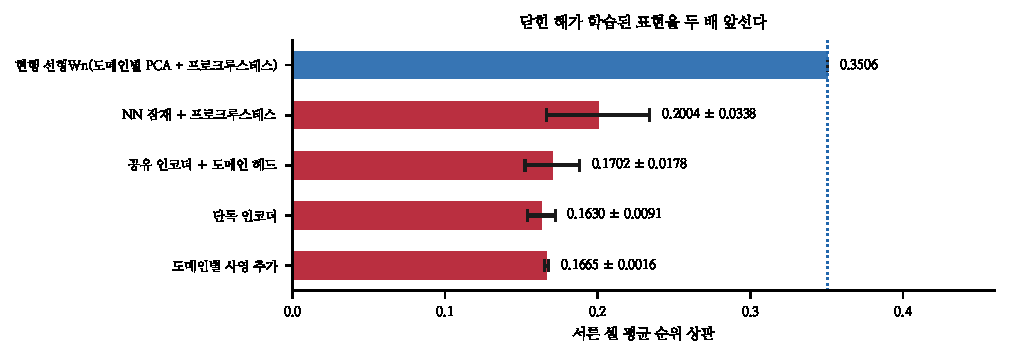
\includegraphics[width=\textwidth]{figs/encoder.pdf}
\caption{서른 셀 평균 순위 상관. 오차 막대는 씨앗 표준편차다.}
\end{figure}

\begin{table}[t]
\centering\tsize
\caption{구성별 성적. 신경망은 씨앗 다섯(또는 셋) 개.}
\begin{tabular}{lr}
\toprule
구성 & 평균 $\rho$ \\
\midrule
\textbf{현행 선형}(도메인별 PCA $+$ 프로크루스테스) & \textbf{$+$0.3506} \\
NN 잠재 $+$ 프로크루스테스 & $+$0.2004 $\pm$ 0.0338 \\
공유 인코더 $+$ 도메인 헤드 & $+$0.1702 $\pm$ 0.0178 \\
도메인별 사영 추가 & $+$0.1665 $\pm$ 0.0016 \\
단독 인코더 & $+$0.1630 $\pm$ 0.0091 \\
\bottomrule
\end{tabular}
\end{table}

차이가 씨앗 표준편차의 10--20배다. \textbf{이번에는 판정할 수 있다.} 노트 14에서
신경망 씨앗 분산이 효과 크기의 4--5배라 아무것도 말할 수 없었는데, 도메인이
여섯이고 레코드가 2,181건이 되면서 씨앗 분산이 0.009--0.018로 내려왔다.

\paragraph{공유가 단독보다 조금 낫다}
$+$0.1702 대 $+$0.1630이다. 다른 도메인에서 배운 표현이 도움이 되긴 한다.
다만 그 이득($+$0.007)이 선형과의 격차($-$0.180)에 비해 미미하다.

\section{원인을 두 번 짚었다}

\paragraph{첫째 가설 --- 회전 자유도}
프로크루스테스는 도메인마다 다른 회전을 허용하고 공통 축 적재로만 맞춘다.
공유 인코더는 모든 도메인을 같은 함수에 통과시키므로 회전이 하나로 강제된다.
그렇다면 도메인별 선형 사영을 인코더 앞에 붙이면 회복돼야 한다.

\begin{table}[t]
\centering\tsize
\caption{도메인별 사영을 앞에 붙였을 때.}
\begin{tabular}{lr}
\toprule
사영 없음 & $+$0.1651 $\pm$ 0.0365 \\
사영 있음 & $+$0.1665 $\pm$ 0.0016 \\
\bottomrule
\end{tabular}
\end{table}

\textbf{변화가 없다. 기각한다.}

\paragraph{둘째 --- 정렬을 되돌려 준다}
신경망을 특징 추출기로만 쓰고, 잠재에 대해 현행과 같은 처리를 했다 --- 공통 축
적재를 도메인마다 계산해 프로크루스테스로 맞춘 뒤 출처 회귀를 적용한다.

$+$0.2004로 \textbf{$+$0.030 회복}한다. 그러나 현행과는 여전히 $+$0.150 차이다.

\claimx{신경망은 표현과 정렬 둘 다에서 진다. 정렬을 프로크루스테스로 되돌려
주면 $+$0.03 회복하고, 나머지 $+$0.15는 표현 자체의 차이다 --- 도메인별 주성분이
공유 인코더보다 낫다.}{잠재 차원을 둘로 묶은 것이 불리했을 수 있다. 넷이나
여덟로 늘리면 표현 격차가 줄 수 있고, 그러면 ``용량을 맞췄다''는 공정성 전제가
잘못이었던 것이다.}

\section{왜 이 문제에서 불리한가}

\begin{itemize}[leftmargin=1.1em,itemsep=0.2em]
\item \textbf{표본이 작다.} 도메인당 62--900건이다. 신경망이 표 형식 데이터에서
      트리나 선형에 지는 전형적인 구간이다(Grinsztajn 2022).
\item \textbf{특징 공학이 이미 끝나 있다.} 입력이 다섯 축뿐이고 그 축은 예순
      노트에 걸쳐 검정으로 다듬은 것이다. 신경망이 찾을 상호작용이 별로 없다.
\item \textbf{도메인마다 축의 관계가 다르다.} 공유 함수는 그것을 하나로 뭉갠다.
      도메인별 PCA는 각자 자기 구조를 잡는다.
\item \textbf{대상 적응이 구조로 주어져 있다.} 현행은 대상 도메인의 데이터로
      대상의 인자 공간과 회전을 만든다. 노트 33의 ``전이 상관 $=$ 대상 자기
      상관''이 바로 그 구조의 결과다.
\end{itemize}

\begin{quote}\fontsize{9.5}{11.5}\selectfont
학습된 공유 표현이 유리해지려면 도메인이 훨씬 많거나 도메인당 표본이 훨씬 커야
한다. 지금 구간에서는 \textbf{닫힌 해가 낫고, 그것을 바꿀 이유가 없다.}
\end{quote}

\section{한계}

\begin{itemize}[leftmargin=1.1em,itemsep=0.15em]
\item 구조 하나(두 층 MLP, 잠재 둘)만 시험했다. 폭 · 깊이 · 정규화를 훑지 않았다.
\item 학습 설정(Adam, lr 3e-3, 400에폭, weight decay 1e-3)을 고정했다. 조정하면
      나아질 수 있고, 조정하면 선택 편향이 들어온다.
\item 짝지은 붓스트랩을 안 붙였다. 차이가 씨앗 SD의 10배 이상이라 필요 없다고
      보았지만 표본 요동은 따로 있다.
\item 도메인 임베딩 · 어텐션 · 사전학습 같은 다른 구성은 안 봤다.
\item 잠재 차원을 늘린 변형을 안 봤다 --- 이 노트의 반증 조건이다.
\end{itemize}

\section{다음}

\begin{enumerate}[leftmargin=1.3em,itemsep=0.15em]
\item 잠재 차원을 넷 · 여덟로 늘려 표현 격차가 줄어드는지 --- 반증 조건.
\item 웹툰 전체 수집 완료 후 전면 재측정(1,315/3,973 진행 중).
\item 보정 표본 층화(노트 59의 남은 항목).
\item 도메인이 열을 넘으면 다시 겨룬다. 지금은 여섯이다.
\end{enumerate}

\vspace{0.6em}
\hrule height 0.3pt
\vspace{0.5em}
{\footnotesize
\textbf{참고문헌}\\[0.3em]
Caruana, R. (1997). Multitask learning. \emph{Machine Learning}, 28(1), 41--75.\\[0.15em]
Maurer, A., Pontil, M., Romera-Paredes, B. (2016). The benefit of multitask
representation learning. \emph{JMLR}, 17(81), 1--32.\\[0.15em]
Grinsztajn, L., Oyallon, E., Varoquaux, G. (2022). Why do tree-based models still
outperform deep learning on typical tabular data? \emph{NeurIPS Datasets and
Benchmarks}.\\[0.15em]
Schönemann, P. H. (1966). A generalized solution of the orthogonal Procrustes
problem. \emph{Psychometrika}, 31(1), 1--10.\\[0.15em]
Bouthillier, X. et al. (2021). Accounting for variance in machine learning
benchmarks. \emph{MLSys}, 3, 747--769.
}

\end{document}
